\chapter{Desenvolvimento} \label{chap:desenvolvimento}

% Citar alguns códigos

Para o desenvolvimento do presente trabalho, foram utilizadas diversas ferramentas, tanto para a elaboração do código, quanto para a elaboração do modelo de banco de dados e para a elaboração do protótipo. Todas elas com o intuito de implementar o software necessário para a criação de uma grade horária.
\section{Projetos anteriores} % ### 5.1.


Antes do desenvolvimento do presente trabalho, foram feitos alguns projetos pessoais que, embora não tenham sido concluídos, serviram como base para o desenvolvimento do presente trabalho.
\subsection{Andamento dos alunos} % #### 5.1.1

Como interesse próprio, cogitou-se o desenvolvimento de uma plataforma onde se pudesse ver em que ponto os alunos se encontram em relação ao andamento de seus cursos. Para isso, seria necessária a obtenção dos dados dos alunos, seja por parte dos mesmos, do coordenador ou por integração com o sistema acadêmico. Com estes dados, seria possível criar uma interface que mostrasse o andamento dos alunos, quais matérias já foram cursadas, quais estão sendo cursadas e quais ainda faltam. Além disso, seria possível mostrar quais matérias são pré-requisitos para outras. Assim, o aluno e a coordenação poderiam ter uma visão geral de seu andamento e de quais matérias ele precisará cursar para se formar. Infelizmente esse projeto não saiu do mundo das ideias. Entretanto, lá permaneceu sendo maturado.


\subsection{Cálculo de demanda} % #### 5.1.2.

Ao longo dos semestres, foi percebido que durante o intervalo entre os semestres, os alunos precisam se inscrever nas matérias que desejam cursar no semestre seguinte. Para isso, é necessário que o coordenador saiba quantos alunos estão interessados em cada matéria para que ele possa definir quantas turmas serão abertas. Com este fim em mente, o coordenador dispõe de algumas alternativas como estimar quantos alunos se inscreverão em cada disciplina, checar manualmente no sistema acadêmico quais alunos podem fazer cada matéria, ou então obter diretamente dos alunos através de um formulário em quais disciplinas cada um dos alunos tem a intenção de cursar.

O método que o atual Coordenador de Ciência da Computação realiza consiste em baixar o extrato de todos os alunos do curso, e tabelar no Excel qual é o andamento de cada um dos alunos, para que assim, através da análise manual pudesse ver qual é o andamento de cada um e de quantos alunos demandam quais disciplinas.

Entretanto, todas essas alternativas são trabalhosas e propensas a erros. Sendo assim, foi pensado em uma forma de automatizar esse processo. Foi então elaborado um código em \href{https://www.python.org/}{Python} que atualmente \href{https://github.com/jvfd3/university_demand}{se encontra no \textit{GitHub}}. Este código tem como entrada os extratos de matrícula dos alunos e como saída a listagem das disciplinas demandadas e a listagem dos alunos que demandam cada disciplina.

\lstinputlisting[language={Python}, captionpos={t}, label={code:demand}, caption={Obter demanda por extratos em PDF}]{files/codigos/demanda.py}

Este código foi desenvolvido em 8 etapas, vistas no \autoref{code:demand}, cada uma com um arquivo separado. Para alcançar a lista das demandas, é necessário primeiro obter a lista dos arquivos em formato PDF que serão processados, em seguida extrair seus dados com a biblioteca \href{https://pypi.org/project/pdfminer/}{\textit{PDFMiner}}, estruturar os dados obtidos, filtrar os dados estruturados, obter a demanda de cada disciplina, juntar as demandas de cada disciplina e salvar os dados obtidos em um arquivo de texto.

Embora o código cumpra com seu objetivo, apresenta algumas características limitantes. A primeira é que os PDFs precisam ser obtidos manualmente, um por um, pelo coordenador, sendo ela por si só uma tarefa extenuante, o que não é desejado. Além disso, o seu uso não é muito intuitivo, sendo necessário que o usuário lide com o prompt de comando e instale as dependências necessárias, o que acaba trazendo uma dificuldade a mais ao usuário. O código também apresenta limitações por sistema operacional, não sendo garantido o seu funcionamento em sistemas operacionais diferentes do Windows.

Com estes empecilhos, o código acabou abandonado, visto que apesar de útil, não era prático o suficiente para ser utilizado.

\section{Dados pessoais e a LGPD} % ### 5.2.

Em sua concepção original, o presente trabalho visaria integrar o sistema desenvolvido com o atual sistema acadêmico da UENF. Essa abordagem foi descartada devido às dificuldades encontradas por parte do setor administrativo da UENF que, devido à \href{https://www.planalto.gov.br/ccivil_03/_ato2015-2018/2018/lei/l13709.htm}{Lei Geral de Proteção dos Dados (LGPD)}, não podem divulgar dados dos alunos, mesmo anonimizados.

Para confirmação das informações recebidas, a \href{https://www.planalto.gov.br/ccivil_03/_ato2015-2018/2018/lei/l13709.htm}{LGPD} foi estudada e talvez o presente estudo recaísse na alínea b do inciso 2º do artigo 4º do capítulo 1 da Lei Nº 13.709, de 14 de agosto de 2018. Informando este que esta lei, a LGPD, não se aplica ao tratamento de dados pessoais realizado para fins exclusivamente acadêmicos.

Segundo o \href{https://www.gov.br/anpd/pt-br/assuntos/noticias/sei_00261-000810_2022_17.pdf}{Estudo Técnico sobre o tratamento de dados pessoais para fins acadêmicos}, é reforçado que ``o tratamento de dados pessoais para fins acadêmicos deve ser sempre lícito''.

Apesar das possibilidades de meios legalmente válidos para a aquisição dos dados, optou-se por abandonar a integração com o Sistema Acadêmico e o uso de dados reais dos alunos já existentes na plataforma. Rumando-se então para uma abordagem mais manual de inserção de dados manualmente por parte dos usuários do sistema.

\section{Prototipagem} % ### 5.3.

\begin{MyCenteredFigure}
  \caption{Protótipos de cartões de turma}
  \label{fig:cartão_de_turma}
  % \hfill
  \begin{minipage}{0.48\textwidth} \centering
    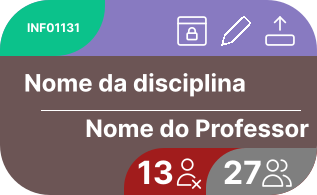
\includegraphics[width=\textwidth]{files/img/Desenvolvimento/Cartões/PadraoClassCards}
    \vspace{1mm} \vfill
    
\includegraphics[width=\textwidth]{files/img/Desenvolvimento/Cartões/Smaller ColapsadaClassCards}
  \end{minipage}
  \hfill
  \begin{minipage}{0.48\textwidth} \centering
    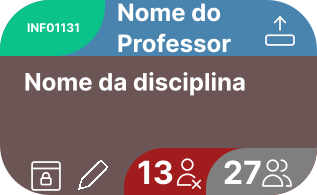
\includegraphics[width=\textwidth]{files/img/Desenvolvimento/Cartões/Professor SuperiorClassCards}
    \vspace{1mm} \vfill
    
\includegraphics[width=\textwidth]{files/img/Desenvolvimento/Cartões/SmallestClassCards}
  \end{minipage}
\end{MyCenteredFigure}
\begin{MyCenteredFigure}
  \caption{Protótipos de Caixas de Seleção}
  \label{fig:selects}
  \begin{minipage}{0.48\textwidth} \centering
    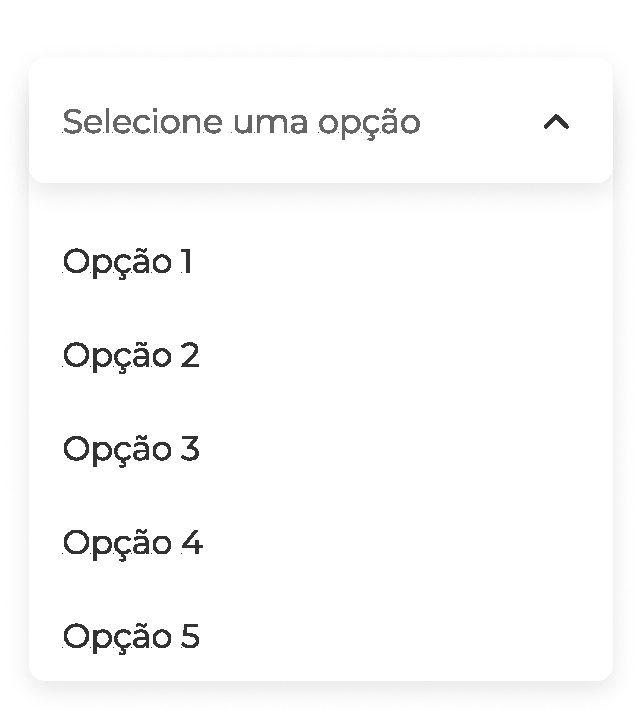
\includegraphics[width=\textwidth]{files/img/Desenvolvimento/SingleSelect.pdf}
  \end{minipage}
  \begin{minipage}{0.48\textwidth} \centering
    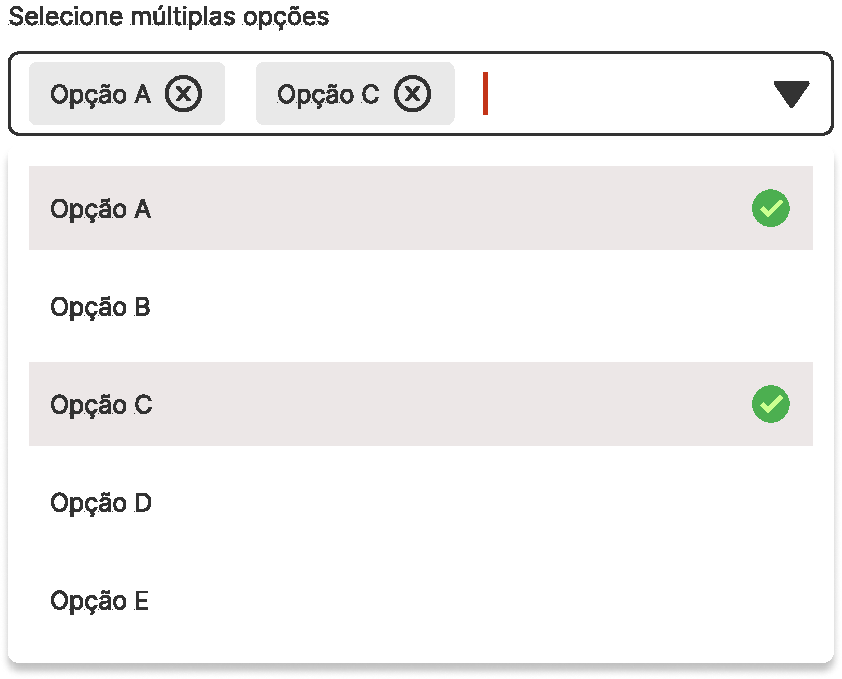
\includegraphics[width=\textwidth]{files/img/Desenvolvimento/MultiSelect.pdf}
  \end{minipage}
\end{MyCenteredFigure}

A criação de protótipos, seguindo a abordagem tomada por \cite{andre_interaction_2018}, se mostra como essencial para que se mantenha a constante satisfação por parte dos \textit{stakeholders} e quais mudanças sugerem ao desenvolvimento do projeto, assim reduzindo a necessidade de retrabalho ou de não alcance das expectativas do projeto.

Para este fim, foram feitos os designs iniciais usando o software de design \href{https://www.figma.com/}{Figma}. Algumas telas principais foram concebidas. A primeira, e principal, é a ilustrada pela \autoref{fig:main} que permite que o usuário arraste a turma até o horário desejado. A turma ao qual este horário se refere pode ser definida na parte lateral direita.
\subsection{Protótipos de páginas} % #### 5.3.1.


\begin{MyCenteredFigure}
  \caption{Página principal do sistema}
  \label{fig:main}
  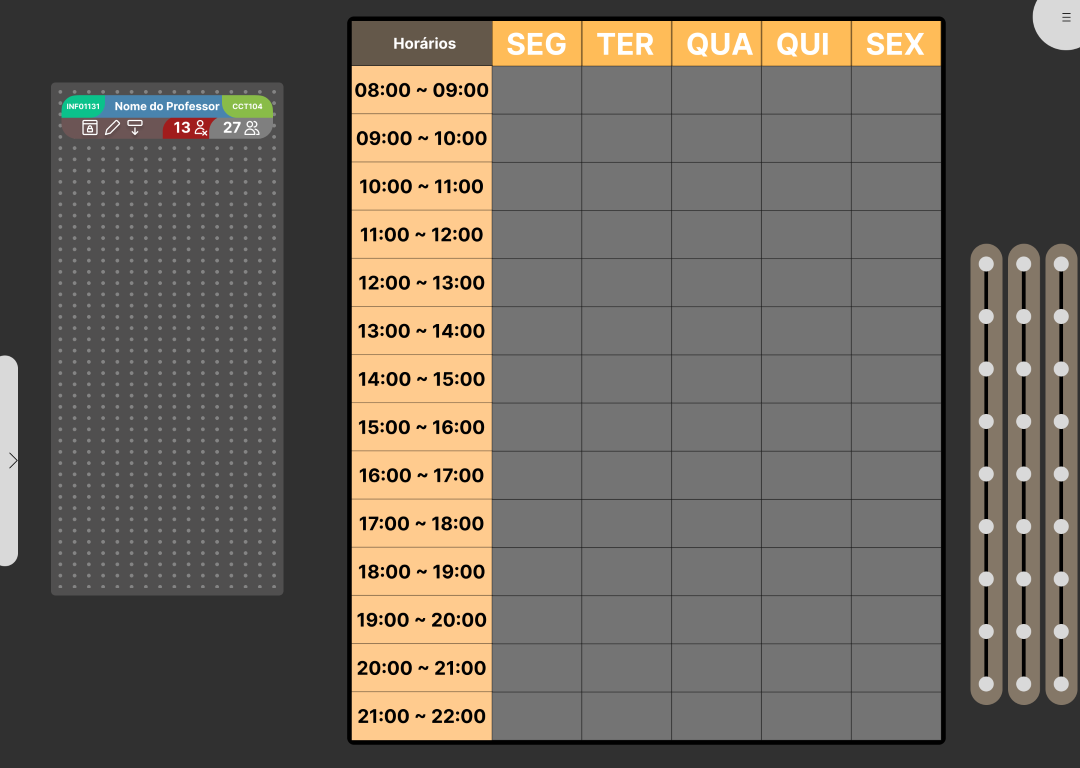
\includegraphics[width=0.8\textwidth]{files/img/Prototipo/Medio/main}
\end{MyCenteredFigure} % Main

Em seguida, temos a tela base para seleção de dados que deseja-se modificar, ilustrada pela \autoref{fig:CRUD_main}, podendo ser de turmas, salas, disciplinas, professores, alunos.

Cada um desses tendo sua própria página de criação, leitura, edição ou deleção de dados.

\begin{MyCenteredFigure}
  \caption{Página principal de modificação dos dados}
  \label{fig:CRUD_main}
  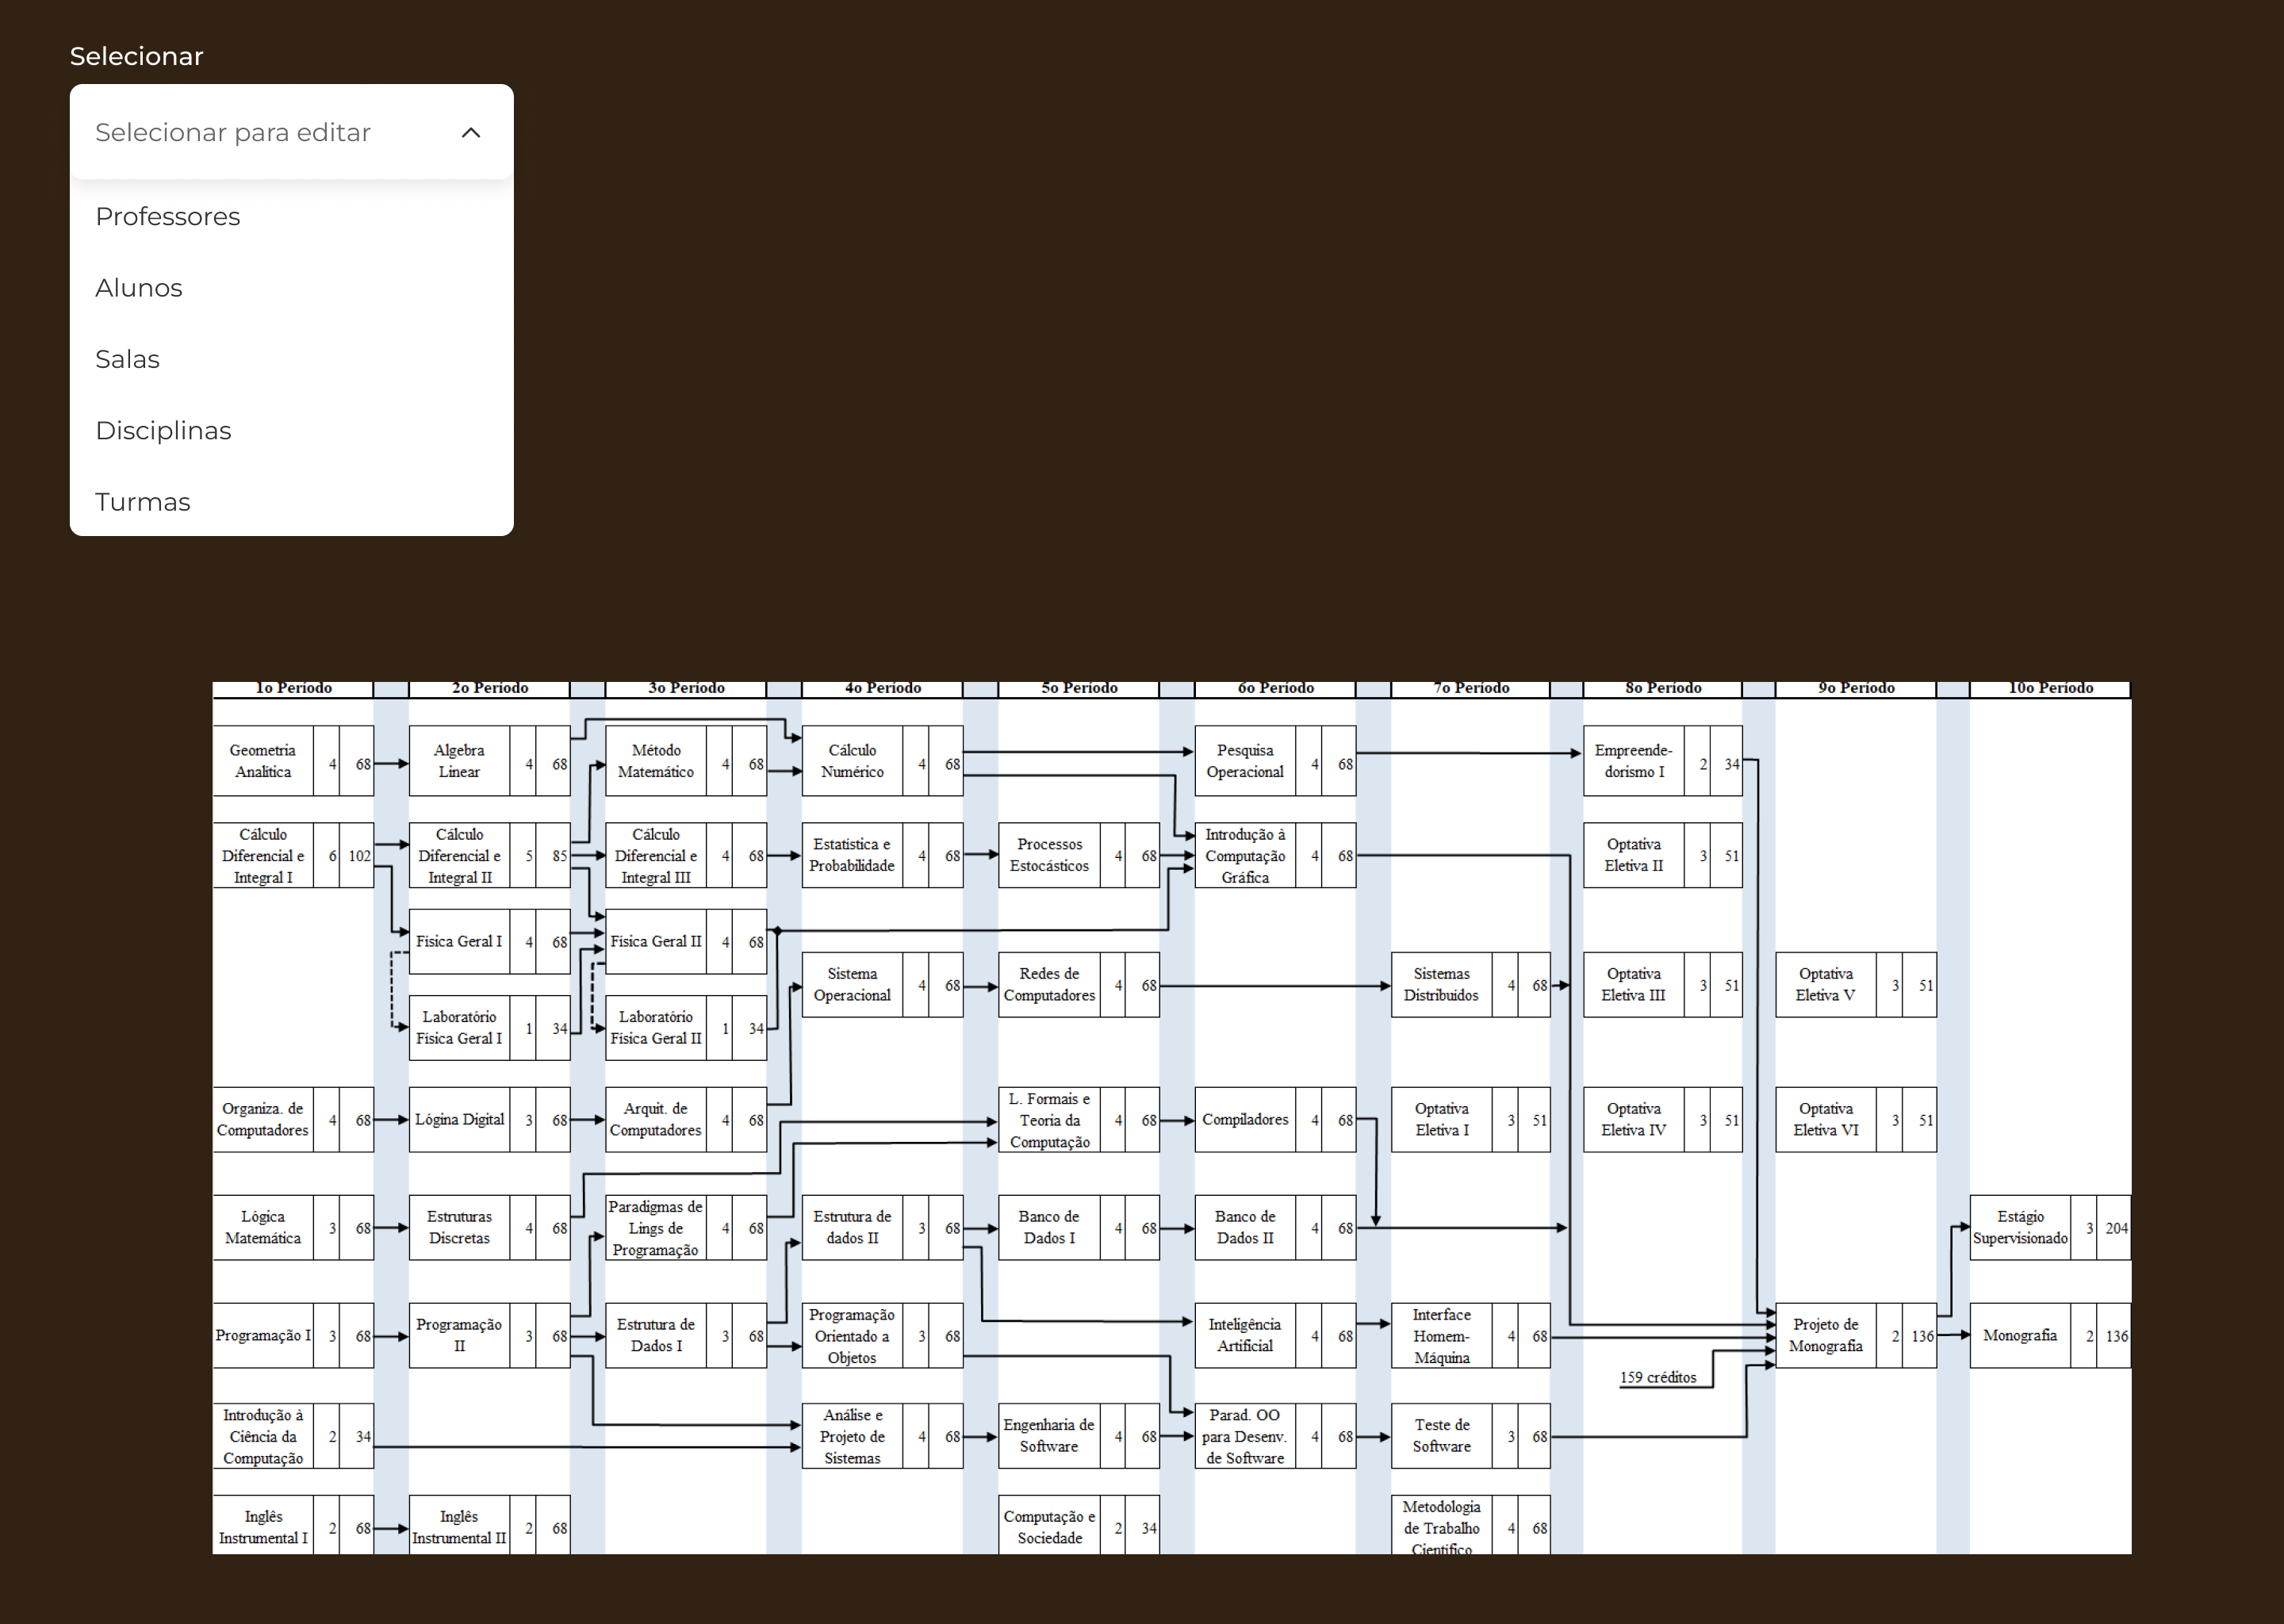
\includegraphics[width=0.8\textwidth]{files/img/Prototipo/Medio/CRUD_main}
\end{MyCenteredFigure} % CRUD_main

Quanto às salas, temos a sua alocação atual baseado no ano e semestre. Nessa página pode-se também registrar algumas características da sala, como a quantidade de cadeiras e computadores, e se possui monitor, projetos, quadro de giz e quadro branco. Um exemplo de sala ainda sem turmas alocadas é representado na \autoref{fig:CRUD_salas-vazias}.

\begin{MyCenteredFigure}
  \caption{Página de modificação das informações de salas}
  \label{fig:CRUD_salas-vazias}
  \includegraphics[width=0.8\textwidth]{files/img/Prototipo/Medio/CRUD_salas-vazias}
\end{MyCenteredFigure} % CRUD_salas-vazias

Na página dos alunos, pode-se cadastrar novos alunos informando o seu ano de entrada e a sua matrícula. Abaixo temos a visualização da grade, onde pode-se classificar cada uma das disciplinas como aprovada, reprovada e cursando. O exemplo da \autoref{fig:CRUD_alunos} mostra a grade de um aluno inscrito em 2019.1.

\begin{MyCenteredFigure}
  \caption{Página de modificação das informações de alunos}
  \label{fig:CRUD_alunos}
  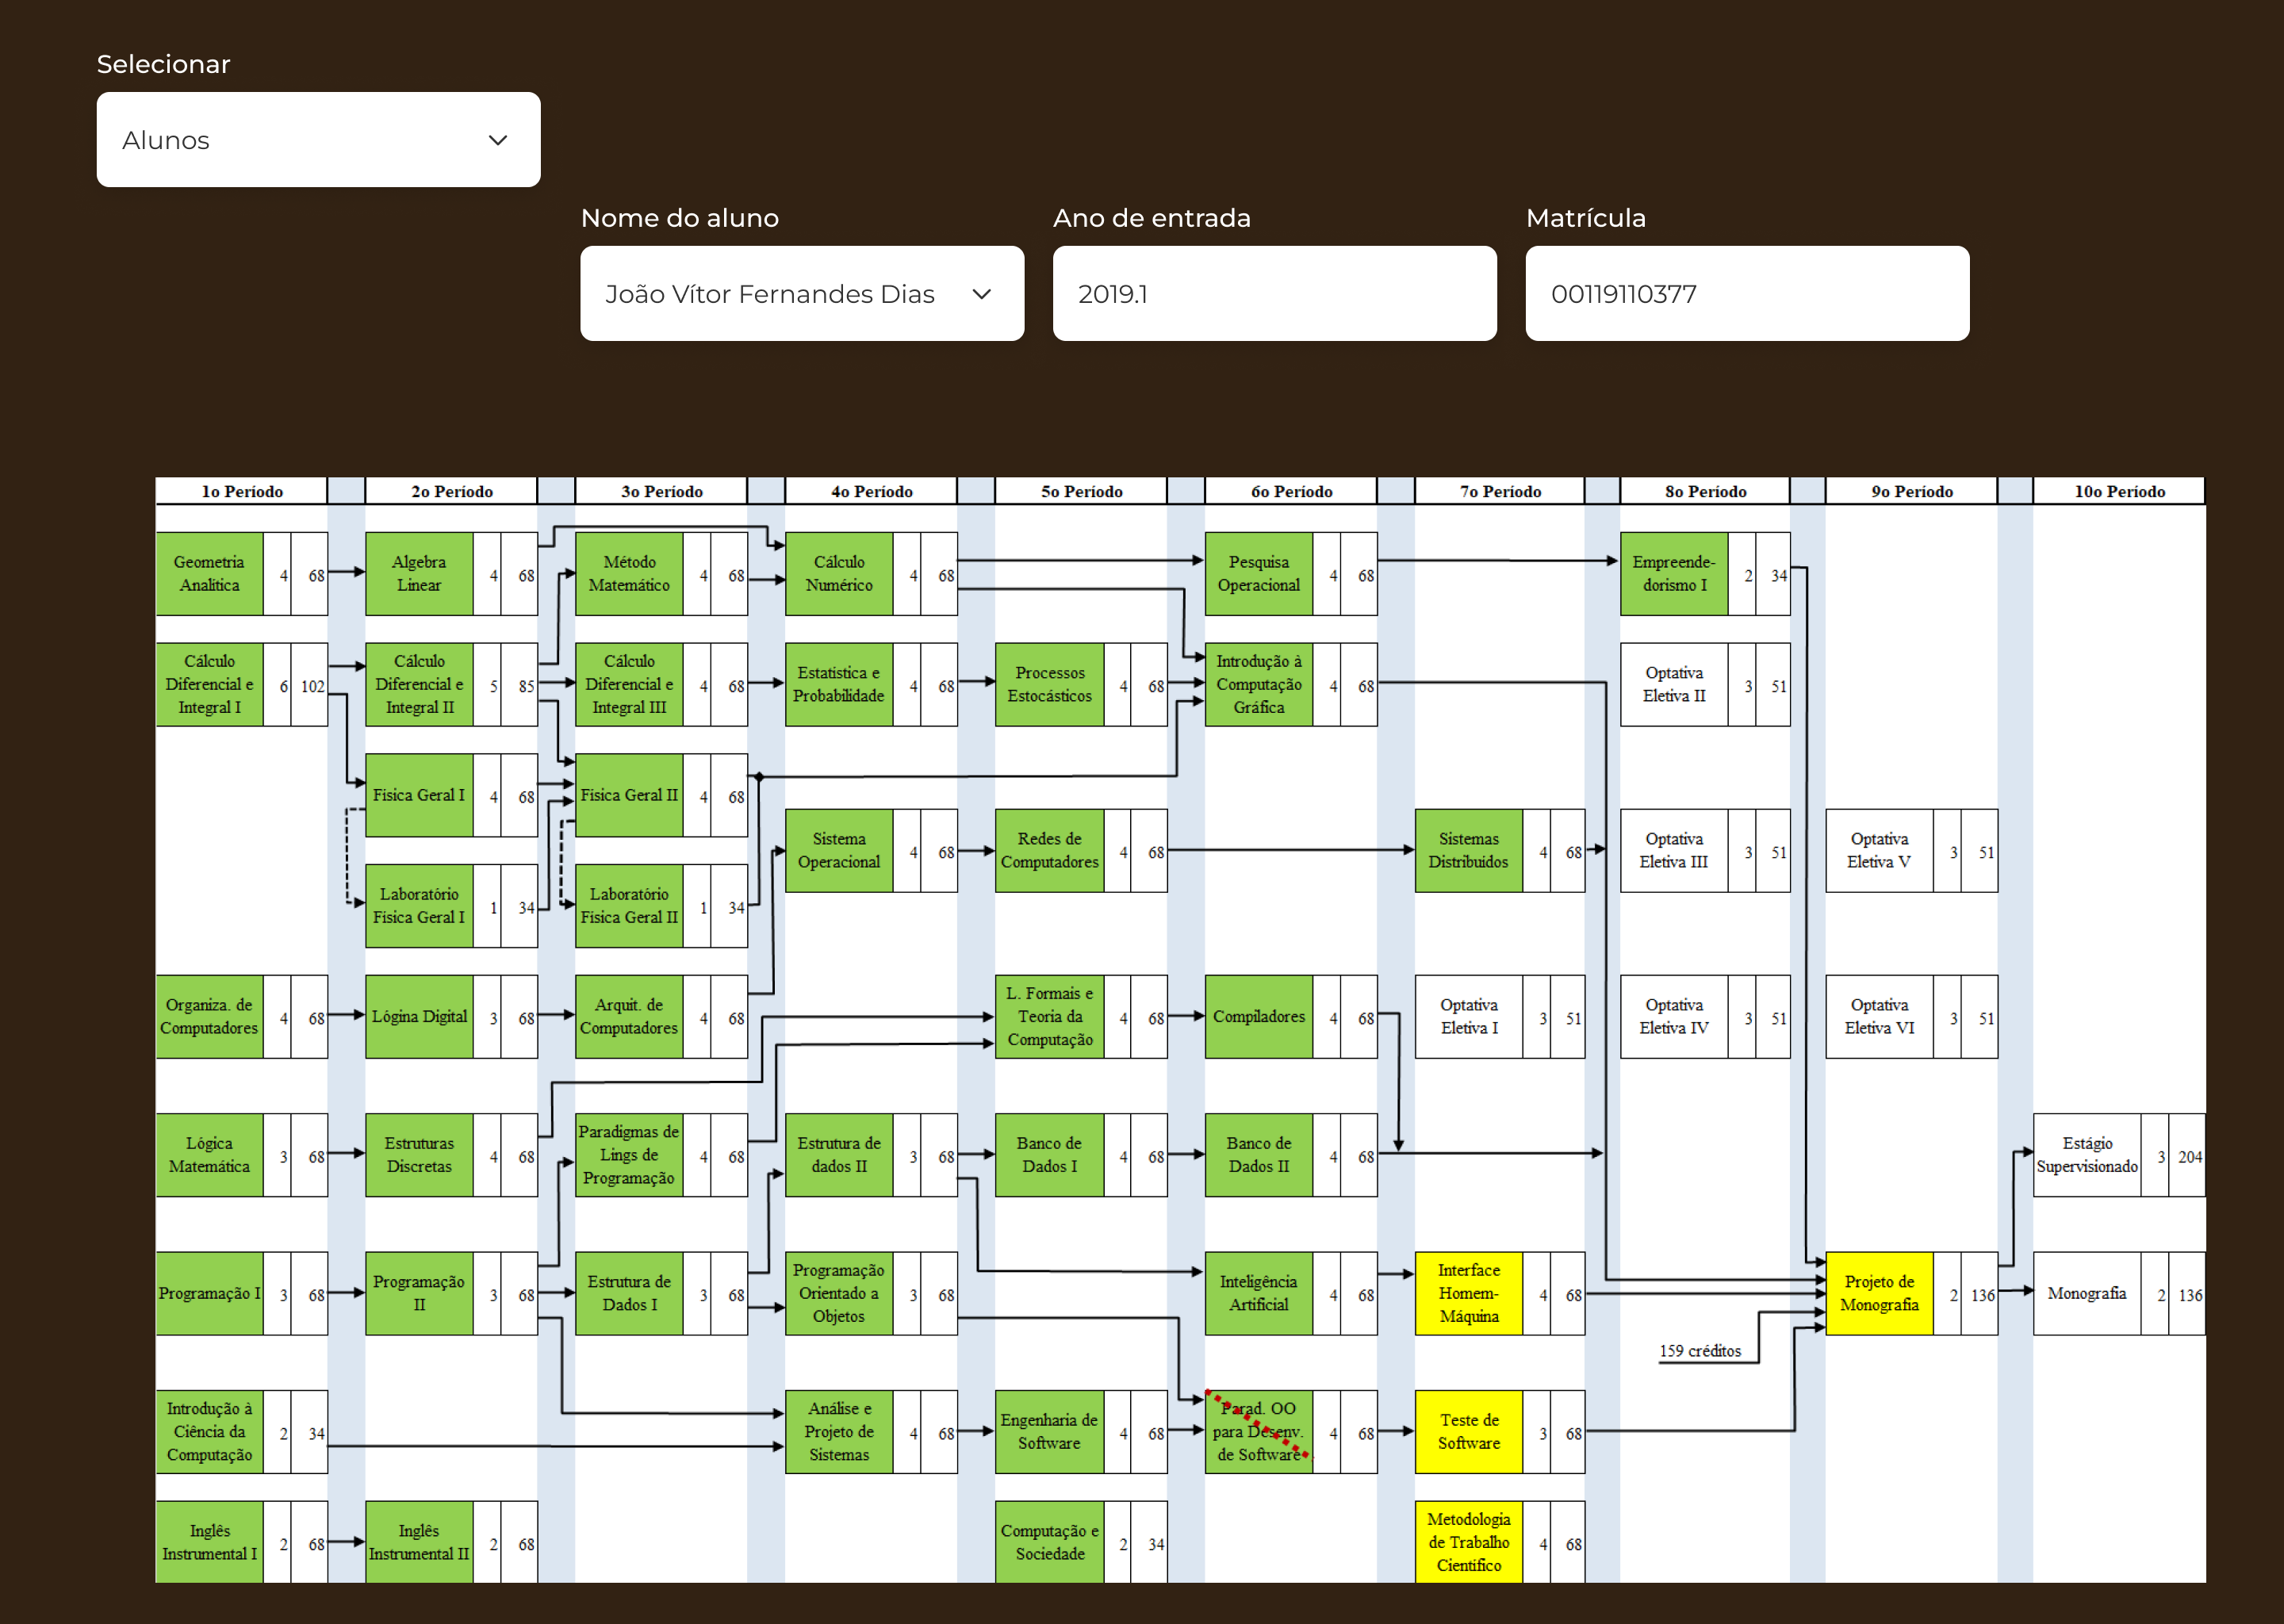
\includegraphics[width=0.8\textwidth]{files/img/Prototipo/Medio/CRUD_alunos}
\end{MyCenteredFigure} % CRUD_alunos

Podemos também definir nas disciplinas qual seu código e nome, e o seu período esperado segundo a ementa. Informamos quais cursos a possuem em suas ementas, quais seus pré-requisitos, os professores que a ministram e quais requisitos a mesma possui em relação às características de sala. A \autoref{fig:CRUD_disciplinas} mostra a página de modificação de disciplinas.

\begin{MyCenteredFigure}
  \caption{Página de modificação das informações de disciplinas}
  \label{fig:CRUD_disciplinas}
  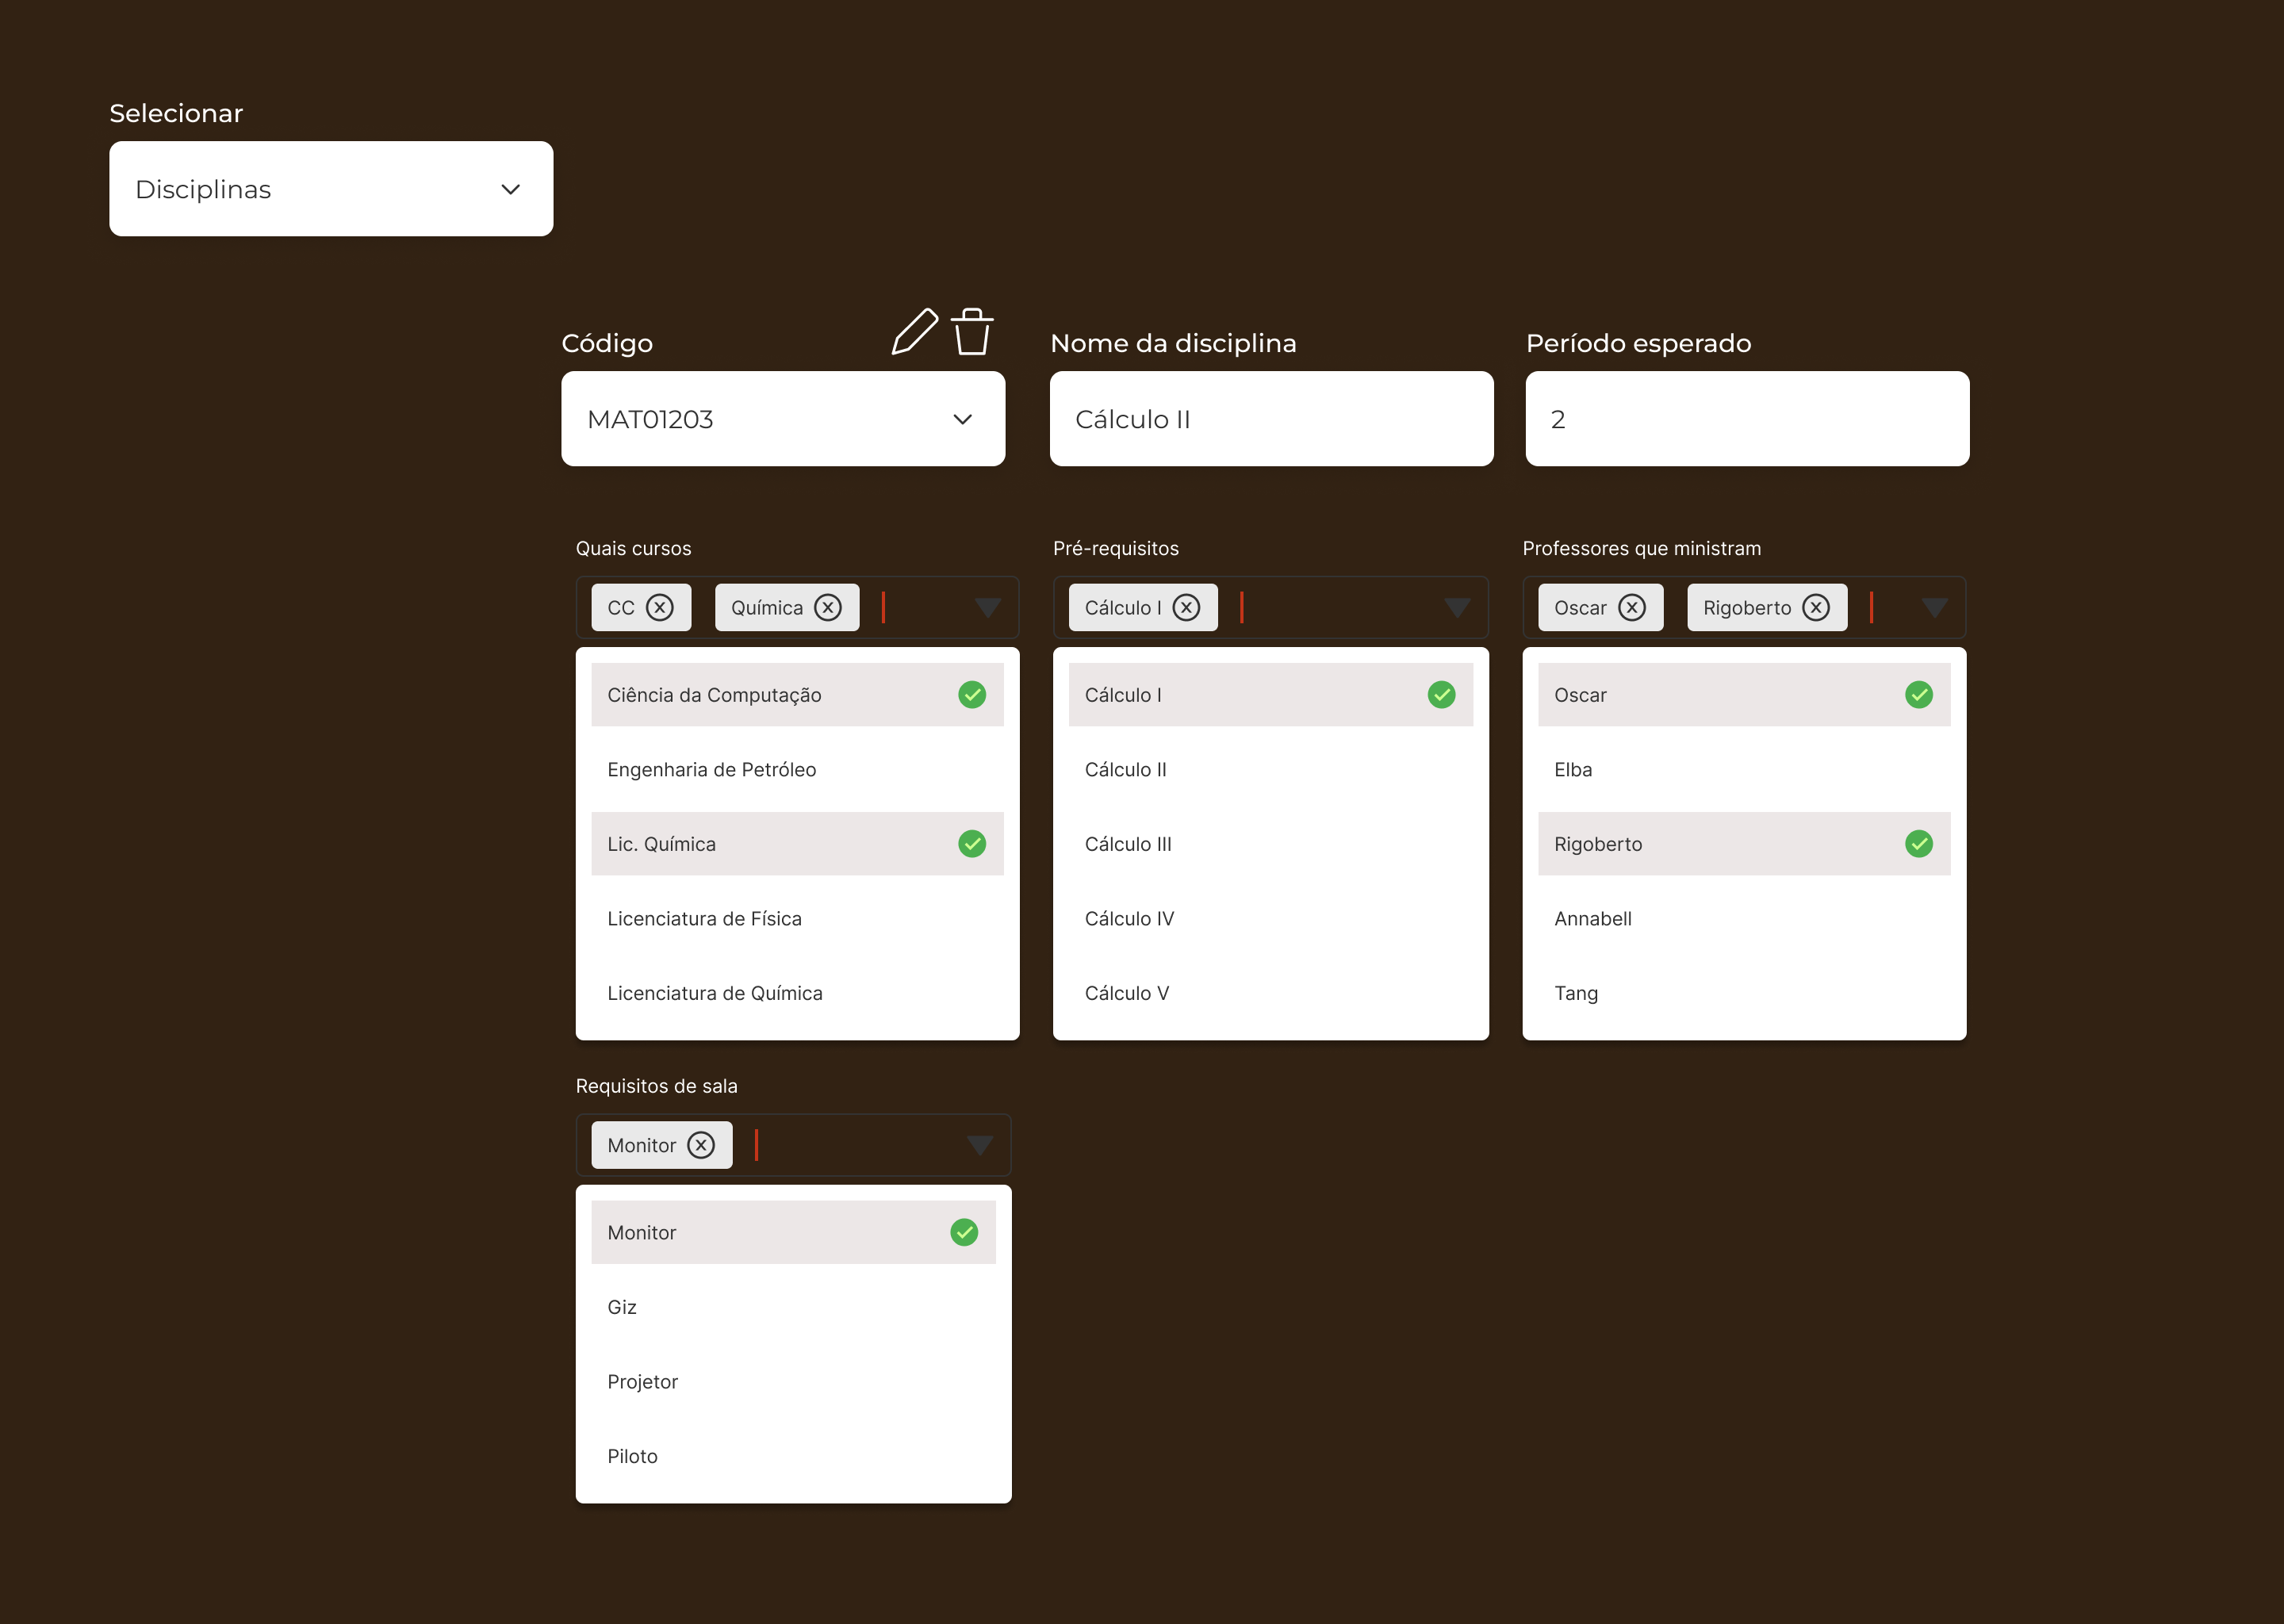
\includegraphics[width=0.8\textwidth]{files/img/Prototipo/Medio/CRUD_disciplinas}
\end{MyCenteredFigure} % CRUD_disciplinas

Na seção de professores, temos a relação de disciplinas que os mesmos estão passíveis de ministrar, e também quais são suas preferências de horários ao longo da semana. A \autoref{fig:CRUD_professores} mostra a página de modificação de professores.

\begin{MyCenteredFigure}
  \caption{Página de modificação}
  \label{fig:CRUD_professores}
  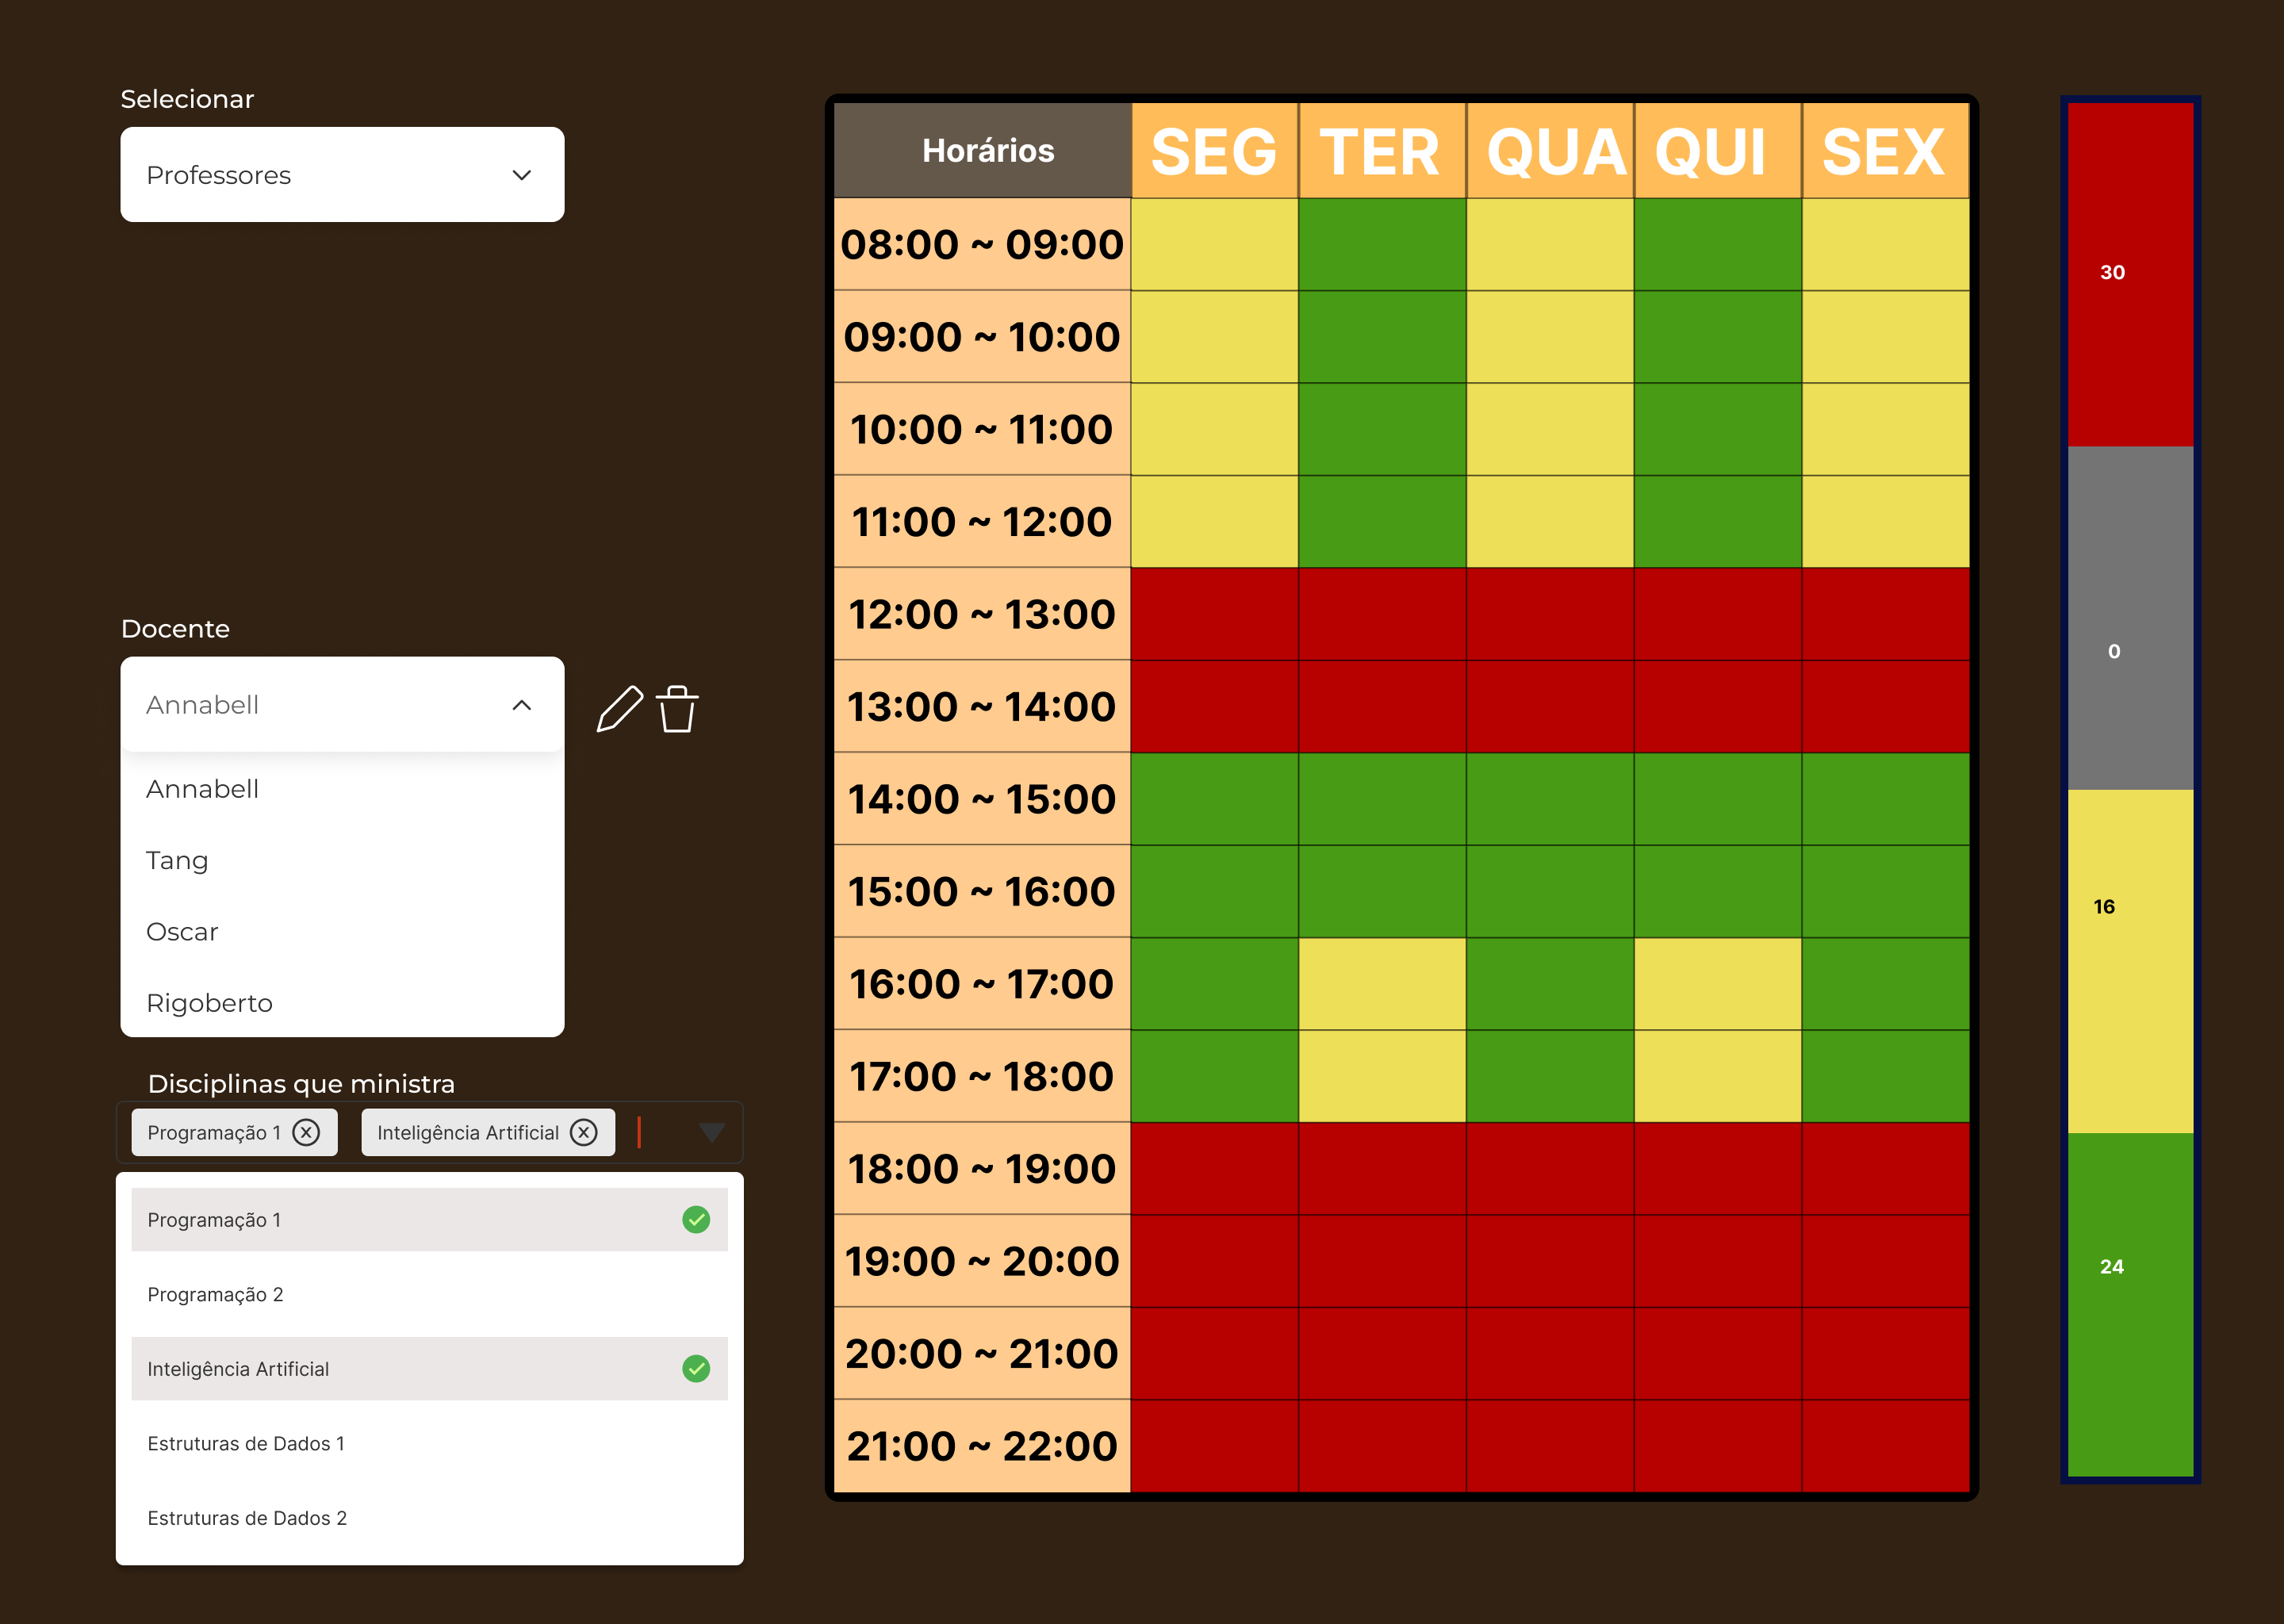
\includegraphics[width=0.8\textwidth]{files/img/Prototipo/Medio/CRUD_professores}
\end{MyCenteredFigure} % CRUD_professores

Por fim, temos a junção de todas as informações registradas acima. Nela, podemos informar em quais horários, dias e em que sala, a turma estará alocada, além de informar qual professor a lecionará e a qual disciplina ela se refere.

Na imagem temos um exemplo das ilustrações de níveis de alerta, informando que o tempo de duração do segundo dia de aulas não condiz com a preferência pessoal do professor selecionado, e que na primeira sala estão ocorrendo conflitos. Conflitos esses ressaltados nos nomes dos alunos que demandam tal disciplina, como pode ser visto na \autoref{fig:CRUD_turmas}.

\begin{MyCenteredFigure}
  \caption{Página de modificação das informações de turmas}
  \label{fig:CRUD_turmas}
  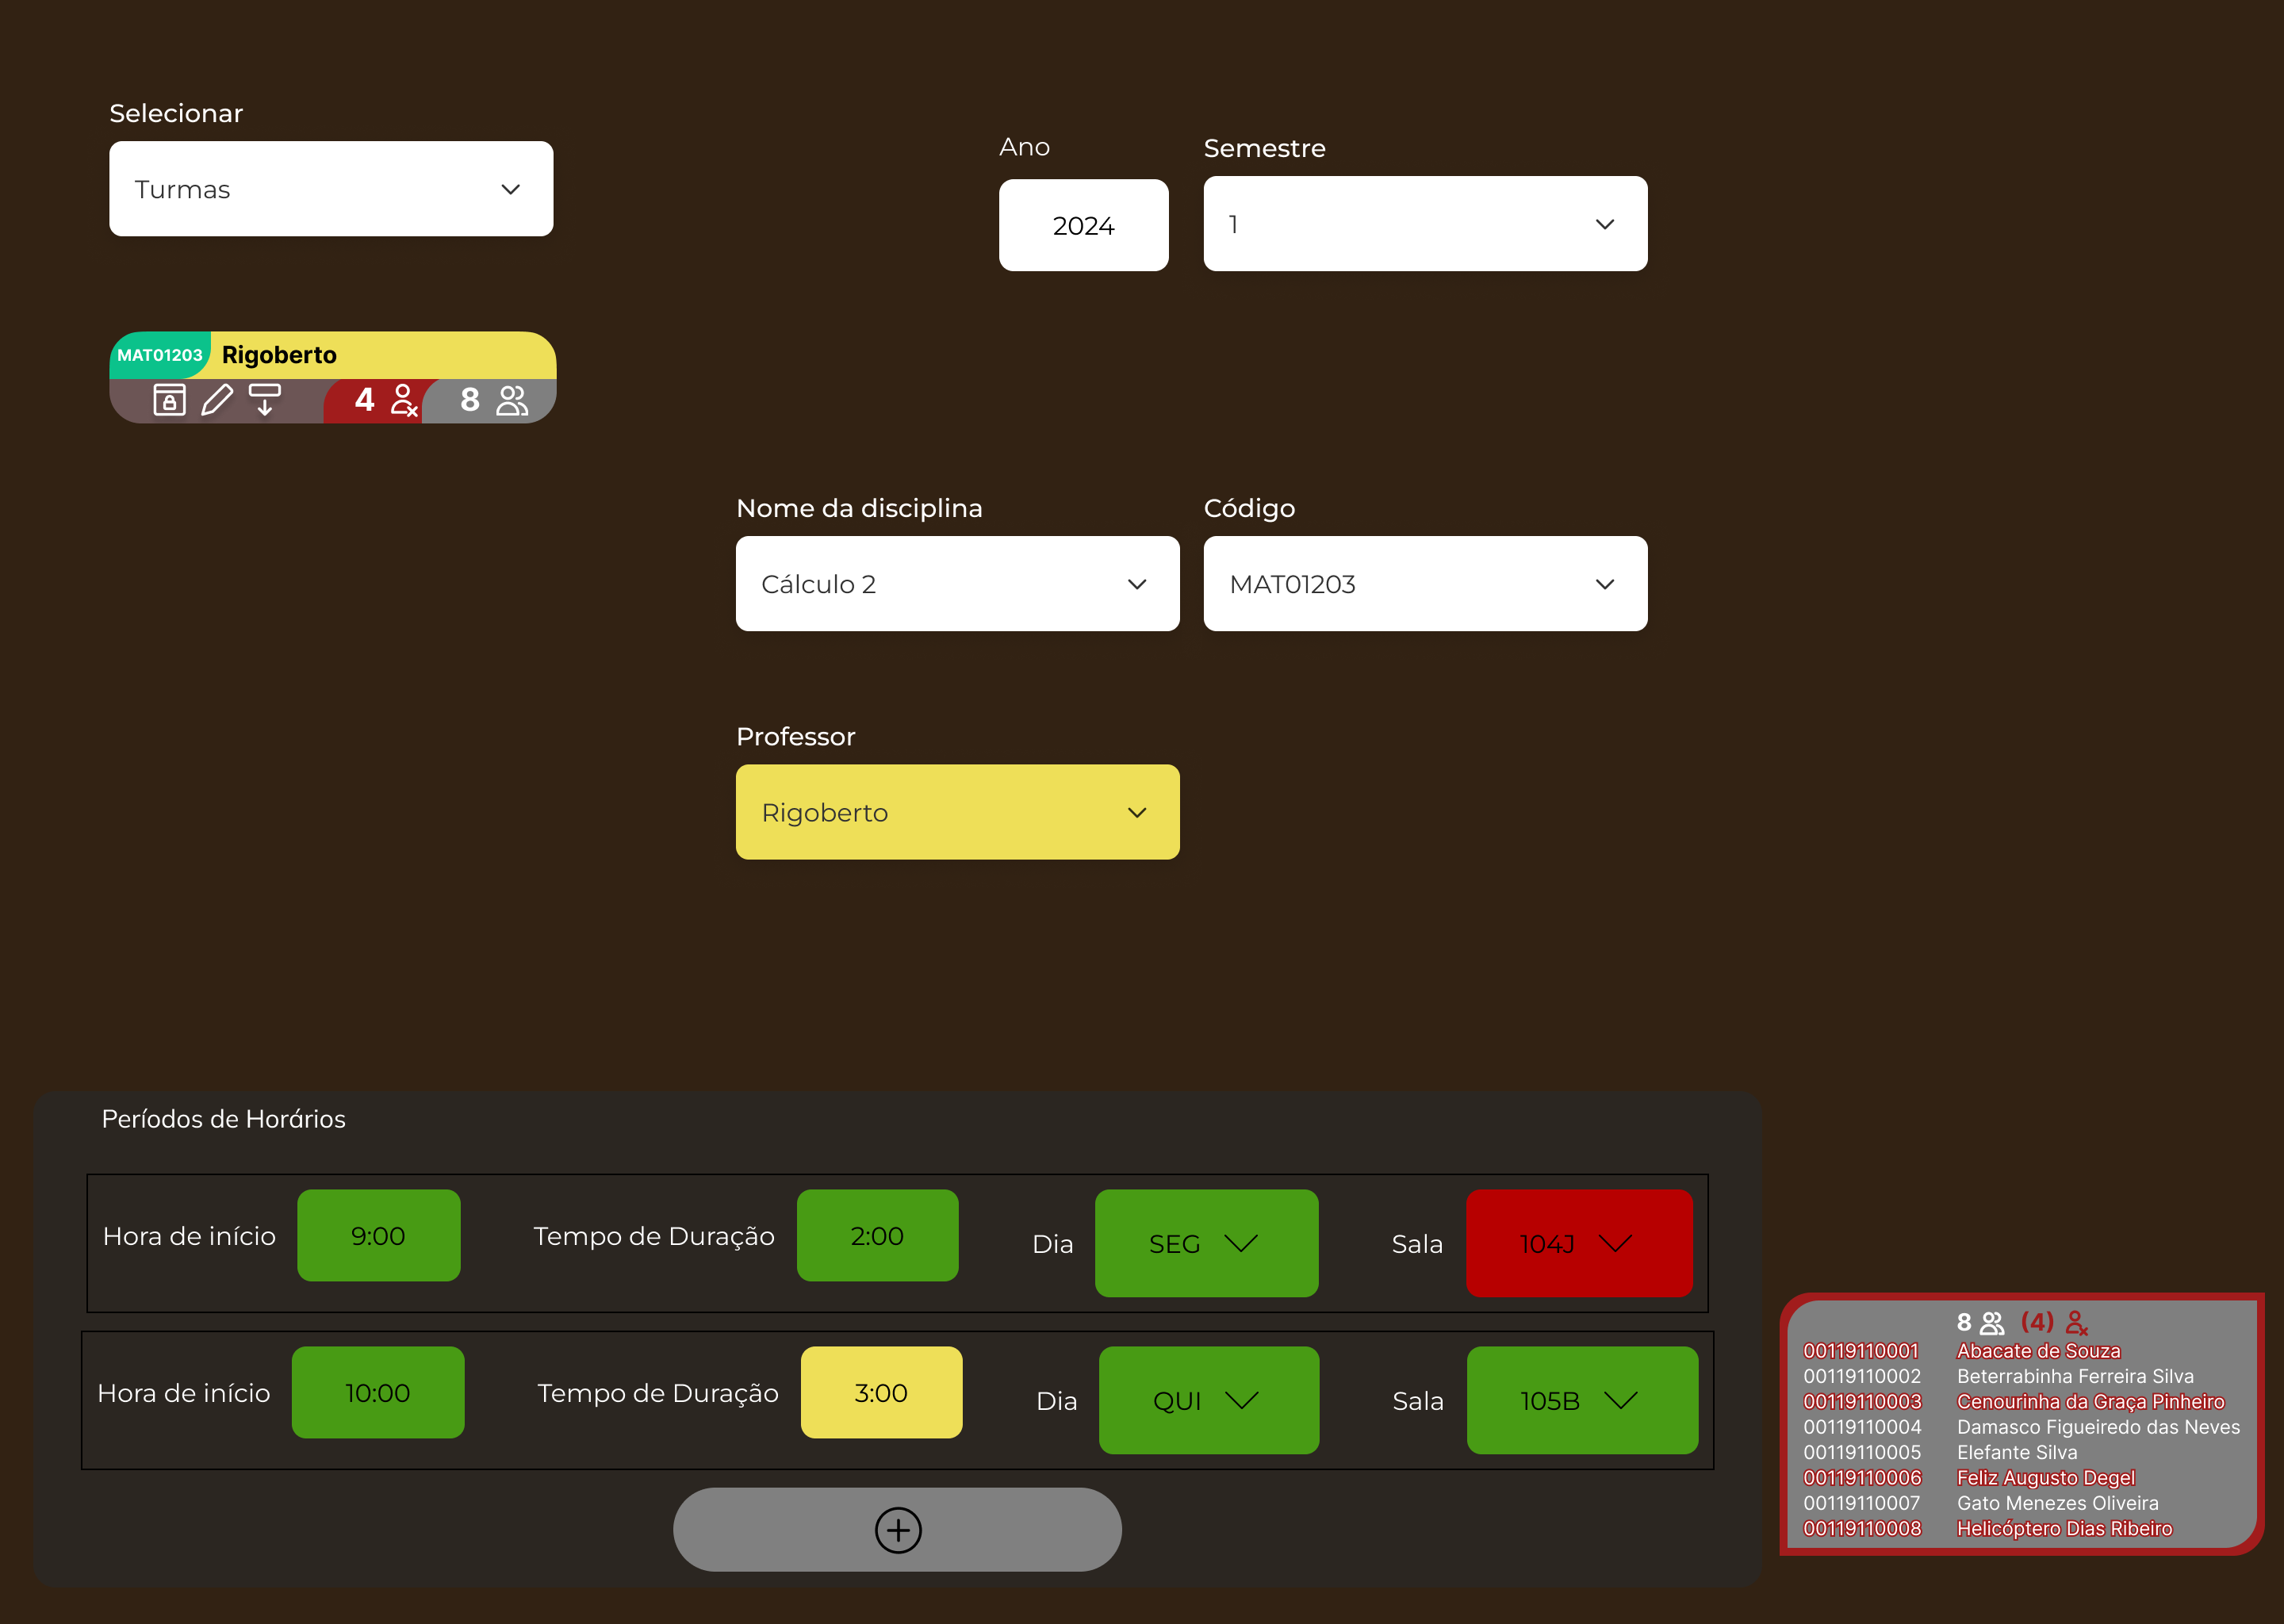
\includegraphics[width=0.8\textwidth]{files/img/Prototipo/Medio/CRUD_turmas}
\end{MyCenteredFigure} % CRUD_turmas
